\section{\textbf{Dependence on Parameters and Initial Conditions}}

\noindent Consider the perturbed system with solution $z(t)$ to the following IVP

\[ \dot{z} = f(z) + g(z) \quad\quad z(t_0) = z_0 \]

\noindent We construct $g(z)$ such that the mass of the drone is doubled, representing a parameter perturbation. We also introduce a perturbation in the initial condition $z_0$.

\[ g(z) = \begin{bmatrix}
    0 \\
    (u_1 + u_2)\sin\theta / 2m \\
    0 \\
    -(u_1 + u_2)\cos\theta / 2m \\
    0 \\
    0
\end{bmatrix} \]

\noindent with the resulting dynamics

\[ \dot{z} = \begin{bmatrix}
    \dot{x} \\
    -(u_1 + u_2) \sin\theta / 2m \\
    \dot{y} \\
    (u_1 + u_2) \cos\theta / 2m - g \\
    \dot{\theta} \\
    r(u_1 - u_2) / I
\end{bmatrix}  \]

\noindent From this, we can compute a $\mu$ used to exponentially bound the growth error such that $||g(z)|| \leq \mu$. Taking the 2-norm:

\[ \begin{aligned}
    \mu &\geq \sqrt{\frac{(u_1+u_2)^2 \cos^2\theta}{4m^2} + \frac{(u_1+u_2)^2 \sin^2\theta}{4m^2}} \\
        &\geq \frac{u_1 + u_2}{2m}
\end{aligned} \]

\noindent For $u_1 = u_2 = u_{max}$, we find $\mu = 10$. By Theorem 3.2 we can construct a bound on the error growth between the nominal solution $x(t)$ and the perturbed solution $z(t)$:

\[ ||x(t) - z(t) || \leq ||x_0 - z_0|| e^{L(t - t_0)} + \frac{\mu}{L}(e^{L(t - t_0)} - 1) \]

\noindent The plot below illustrates that the actual norm of the solution difference remains well below this theoretical exponential bound, confirming the continuous dependence on initial conditions and parameters.\\

\noindent For the initial conditions
\[ x_0 = \begin{bmatrix}
    0 & 0 & 0 & 0 & 0 & 0
\end{bmatrix} \]
\[ z_0 = \begin{bmatrix}
    0 & 1 & 0 & 1 & 0 & 0
\end{bmatrix} \]

\noindent we have the error growth

\begin{figure}[h]
    \centering
    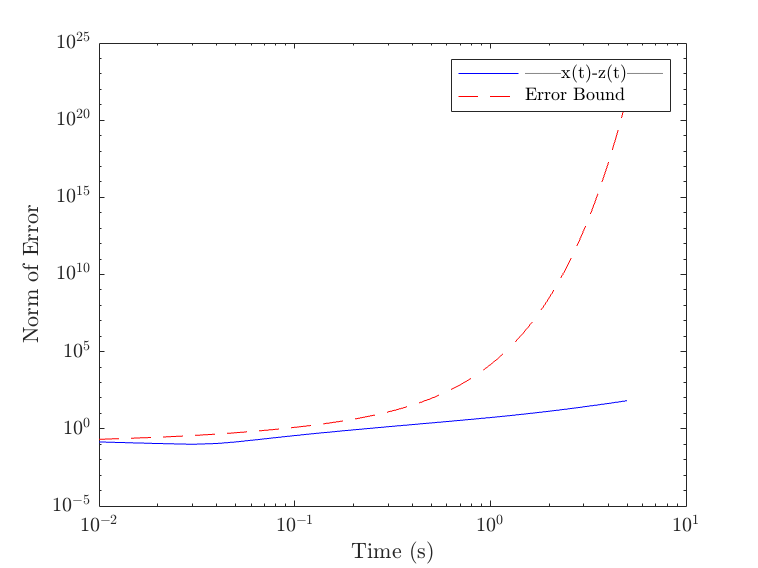
\includegraphics[width=0.75\columnwidth]{figures/cp2/bound.png}
    \caption{Exponential Bound on Error Growth}
    \label{fig:exp_bound}
\end{figure}
